\begin{otherlanguage}{french}
\chapter{R\'esum\'e en Fran\c{c}ais}
\definechapterdirectory{src/summary}

\stopallthesefloats
% INTRO
% 1 page.
% Ce qui est dans l'intro, toute la section 1.1 (Context) et le 1.3
The introduction of multi-core processors in critical avionic systems requires
the ability to sufficiently predict their behavior so that certification of the
system is achievable. Indeed, the parallel nature of multi-core processors
leads to numerous interactions that do not strictly pertain to the objective
of the applications being ran. This large amount of unprompted interactions
render execution times difficult to predict and subject to large variations.
Among the main causes of large time variations is cache coherence, the
mechanism ensuring that data modifications performed by programs running in
parallel are properly propagated. While cache coherence can be implemented with
predictability in mind (see
Section~\ref{sec:rel_work:handling_it:through_hardware}), this requires hardware
modifications, precluding such solutions in an aeronautical context.
Unfortunately, the available strategies to predict worst-case execution time of
applications running on multi-core \textit{Commercial Off-The-Shelf} processors
require cache coherence to be deactivated (see
Section~\ref{sec:rel_work:handling_it:accepting_it} and
Chapter~\ref{cha:analyzing_rel_work}).

This thesis proposes solutions to begin addressing the issue of cache coherence
predictability in an aeronautical context. To do so, it provides the applicant
with tools that can expose and explain the interference generated by cache
coherence. In this chapter is provided a summary, the limitations, and
suggestions of future improvements for each contribution made in this thesis.


\stopallthesefloats

% \section{Prelimnaires}
% 4 pages.
% \subsection{Timed Automata}
% \subsubsection{Definition des timed automata}
% Pas def2
% Mettre la def3, 4, 5, 6. Example 2, 3.
% 
% Juste la def d'un timed automata. Juste le minimum dont on a besoin.
% 
% \subsubsection{UPPAAL et network oto}
% def 9, 11, 12, 13, 14, 15. Example 6.
% 
% \subsection{Fondamental des caches}
% La notationd de l'intro jusqu'a 3.1
% 
% \subsubsection{Composants}
% Resume des composants en une seule sous-section.
% 
% \subsubsection{Resume de MSI}. Pour split-base: juste dire rapidement que
% c'est complique.

\section{Notions pr\'eliminaires}

\subsection{Automates temporis\'es}
\label{fr:sec:formal_methods}
Les automates temporisés seront utilisés dans la suite pour réaliser un modèle formel de
des architectures.
Un automate temporisé est un automate étendu permettant en outre de modéliser le temps, et ce
en ajoutant un nouveau type de variable appelé horloge. On rappelle qu'un automate étendu est un automate
pouvant manipuler des variables entières.


\begin{definition}[Horloges]
  Une \textit{horloge} est une variable modélisant le passage du temps.
  La valeur d'une horloge ne croit que dans les états car les transitions sont instantanées.
  La valeur d'une horloge peut être testée sur une garde d'une transition et remise à zéro après franchissement d'une transition.
\end{definition}


\begin{definition}[Syntaxe des contraintes et des actions]
\label{fr:def:formal_methods:transition_grammar2}
Étant donné un ensemble de variables \automatavariables{}, et un ensemble
d'horloges \automataclocks{}, la grammaire utilisée pour l'écriture des
contraintes et des actions de transitions est la suivante, avec \textbf{ident}
indiquant une variable dans \automatavariables{} et \textbf{clk} une horloge
dans \automataclocks{}:\\
$\textbf{lop} ::= \land~|~\lor $\\
$\textbf{cop} ::=\!\!\! ~< | \le | = | \ge | > $\\
$\textbf{mop} ::= +~| - | * |~/$\\
$
\textbf{val} ::=
   \textbf{ident}
   ~|~ \mathbb{Z}
$\\
$\textbf{mexpr} ::=
   \textbf{mexpr}~\textbf{mop}~\textbf{mexpr}
   ~|~ \textbf{val}
$\\
$
\textbf{abexpr} ::=
   \textbf{mexpr}~\textbf{cop}~\textbf{mexpr}
   ~|~ \textbf{clk}~\textbf{cop}~\textbf{val}
   ~|~ \textbf{clk} - \textbf{clk}~\textbf{cop}~\textbf{val}
   ~|~ \texttt{true}
   ~|~ \texttt{false}
$\\
$
\textbf{bexpr} ::=
   \neg \textbf{bexpr}
   ~|~ \textbf{bexpr}~\textbf{lop}~\textbf{bexpr}
   ~|~ \textbf{abexpr}
$\\
$\textbf{iexpr} ::=
   \textbf{iexpr} \land \textbf{iexpr}
   ~|~ \textbf{clk}~\textbf{cop}~\textbf{val}
   ~|~ \textbf{clk} - \textbf{clk}~\textbf{cop}~\textbf{val}
   ~|~ \texttt{true}
$\\
$
\textbf{assign} ::=
   \textbf{assign};~\textbf{assign}
   ~|~ \textbf{ident}~:=~\textbf{mexpr}
   ~|~ if~(\textbf{bexpr})~\{\textbf{assign}\}
   ~|~ \textbf{clk} := 0
   ~|~ \texttt{nop}
$
\end{definition}



\begin{definition}[Automates temporisés]
Un automate temporisé \automatasystem{} est un tuple
$\langle \automatastates{}, \allowbreak{}
\automatainvariants{}, \allowbreak{}
\automatainit{}, \allowbreak{}
\automatacondlabels{}, \allowbreak{}
\automatachanlabels{}, \allowbreak{}
\automatachanpriorities{}, \allowbreak{}
\automatavariables{}, \allowbreak{}
\automataclocks{}, \allowbreak{}
\automataactionlabels{}, \allowbreak{}
\automatarelations{}\rangle$ tel que:
\begin{itemize}
  \setlength{\itemsep}{0pt}%
   \setlength{\parskip}{0pt}%
\item \automatastates{} est un ensemble fini de localités.
\item
   $\automatainvariants{} : \automatastates{} \to \textbf{iexpr}$ indique
   l'invariant associé à chaque localité.
\item \automatainit{} est la localité initiale ($\automatainit{} \in
\automatastates{}$).
\item \automatavariables{} est un ensemble fini de variables.
\item \automataclocks{} est un ensemble fini d'horloges.
\item
   $\automatachanlabels{} = \automatachanlabels{}^{\alpha} \cup
   \automatachanlabels{}^{\texttt{sync}}$ est un ensemble fini d'étiquettes, avec
   $\automatachanlabels{}^{\texttt{sync}}$ correspondant aux étiquettes de
   synchronisation et $\automatachanlabels{}^{\alpha}$ aux autres.
   $\automatachanlabels{}^{\texttt{sync}} \cap \automatachanlabels{}^{\alpha}
   = \emptyset$.
   Les étiquettes dans $\automatachanlabels{}^{\texttt{sync}}$ terminent soit par
   par `?' qui indique la réception sur un ``canal'',
   ou par `!' qui indique l'émission.
\item
   \automatacondlabels{} = \textbf{bexpr}(\automatavariables{},
   \automataclocks{}) est l'ensemble des gardes, utilisant la grammaire de
   Définition~\ref{fr:def:formal_methods:transition_grammar2}.
\item
   \automataactionlabels{} = \textbf{assign}(\automatavariables{},
   \automataclocks{}), est l'ensemble des actions, utilisant la grammaire de
   Définition~\ref{fr:def:formal_methods:transition_grammar2}.
\item
   $\automatarelations{} \subseteq
      \automatastates{}
      \times \automatacondlabels{}
      \times \automatachanlabels{}
      \times \automataactionlabels{}
      \times \automatastates{}
   $ est la relation de transition.
\end{itemize}
La sémantique de \automatasystem{} est donnée à travers ses traces d'exécution
(voir Définition~\ref{fr:def:formal_methods:trace2}).
\end{definition}

\begin{definition}[Valuation d'horloge]
La fonction
$\automataclockvals{}: \automataclocks \to \mathbb{R}^+$ assigne une valuation
à chaque horloge. On note $(\automataclockvals{} + t)$ comme abréviation pour
indiquer l'incrément de la valeur de toutes les horloges dans \automataclockvals{}
de $t$ unités de temps.
\end{definition}

\begin{definition}[Valuation des variables]
  Les valuations
$\automataenvironment{}:\automatavariables{} \to \mathbb{N}$
  associent aux variables leur valeur.
Étant donné une valuation $\automataenvironment{}$ et une garde
$c \in \automatacondlabels{}$, on note $\automataenvironment{} \models_{PL} c$
pour indiquer que $c$ est vraie selon la valuation $v$.
De même, étant donné $a \in \automataactionlabels{}$, $v[a]$ correspond à la
valuation obtenue depuis $v$ par l'application de l'action $a$: toutes les
variables changées par $a$ ont leur nouvelle valeur et toutes les autres gardent
leur valeur précédente.
\end{definition}


\begin{definition}[Transition]
Étant donné un automate
$\automatasystem{} = \allowbreak{}
\langle \automatastates{}, \allowbreak{}
\automatainvariants{}, \allowbreak{}
\automatainit{}, \allowbreak{}
\automatacondlabels{}, \allowbreak{}
\automatachanlabels{}, \allowbreak{}
\automatachanpriorities{}, \allowbreak{}
\automatavariables{}, \allowbreak{}
\automataclocks{}, \allowbreak{}
\automataactionlabels{}, \allowbreak{}
\automatarelations{}\rangle$,
on définit \automatanext{} permettant de calculer l'ensemble des transitions valides depuis
$\langle \automatastate{}, \automataenvironment{}, \automataclockvals{}\rangle$,
avec
$s \in \automatastates{}$, $\automataenvironment{}$ une valuation des variables,
$\automataclockvals{}$ une valuation des horloges et $t$ le temps passé
dans la localité courante:
$\automatanext{}(\langle \automatastate{}, \automataenvironment{}, \automataclockvals{}\rangle, t)
\triangleq \{\langle \automatastate{}', \automataenvironment{}', \automataclockvals{}' \rangle
|
   \existsin{\langle \automatastate{}, c, l, a, \automatastate{}' \rangle}{\automatarelations{}}{%
%      (o = \automatastate{})
%      \land (d = \automatastate{}')
      (\langle \automataenvironment{}, (\automataclockvals{} + t) \rangle \models_{PL} c)
      \land
      \automataenvironment{}' = \automataenvironment{}[a]
      \land
      \automataclockvals{}' = (\automataclockvals{} + t)[a]
      \land
      (\langle \automataenvironment{}', \automataclockvals{}' \rangle \models_{PL} \automatainvariants{}(\automatastate{}'))
      \land
      \neg
      \existsin{\langle \automatastate{b}, c_b, l_b, a_b, \automatastate{b}' \rangle}{\automatarelations{}}{%
   %      (o = \automatastate{})
   %      \land (d = \automatastate{}')
         (\langle \automataenvironment{}, (\automataclockvals{} + t) \rangle \models_{PL} c_b)
         \land
         \automataenvironment{}'' = \automataenvironment{}[a_b]
         \land
         \automataclockvals{}'' = (\automataclockvals{} + t)[a_b]
         \land
         (\langle \automataenvironment{b}'', \automataclockvals{b}'' \rangle \models_{PL} \automatainvariants{}(\automatastate{b}'))
         \land
         (l \in \automatachanpriorities{}(l_b)) \allowbreak{}
      }
   }\}
$
\end{definition}

\begin{definition}[Chemin et trace]
\label{fr:def:formal_methods:trace2}
Un chemin est une séquence maximale de transitions\linebreak
$\langle \automatastate{0}, \automataenvironment{0}, \automataclockvals{0}\rangle
\automatatransition{}^{\!\!\!t_0} \langle \automatastate{1},
\automataenvironment{1}, \automataclockvals{1}\rangle \automatatransition{}^{\!\!\!t_{1}} \cdots$ telle que pour chaque $k$,
$\langle \automatastate{k+1}, \automataenvironment{k+1}, \automataclockvals{k+1}\rangle \in \automatanext{}(\langle \automatastate{k}, \automataenvironment{k}, \automataclockvals{k}\rangle, t_k)
$.
La séquence est maximale dans le sens où elle est soit infinie soit de longueur $N$ et telle que $\automatanext{}(\langle \automatastate{N}, \automataenvironment{N}, \automataclockvals{N}\rangle, t)$ est vide pour tout $t\in \mathbb{R}^+$. On appelle trace un chemin partant de l'état initial
$\langle
\automatainit{}, \automataenvironment{0},  \automataclockvals{0}\rangle$, avec
\automataenvironment{0} la valuation initiale et \automataclockvals{0} la valuation
telle que toutes les horloges sont à zéro.
\end{definition}


\begin{definition}[Produit synchronisé d'automates temporisés]
Étant donné \emph{n} automates temporisés
$\automatasystem{}_i = \allowbreak{}
\langle \automatastates{}_i, \allowbreak{}
\automatainvariants{}_i, \allowbreak{}
\automatainit{}_i, \allowbreak{}
\automatacondlabels{}_i, \allowbreak{}
\automatachanlabels{}_i, \allowbreak{}
\automatavariables{}_i, \allowbreak{}
\automataclocks{}, \allowbreak{}
\automataactionlabels{}_i, \allowbreak{}
\automatarelations{}_i\rangle$ et une contrainte de synchronisation
$\automatasyncconstraint{} \subseteq (\automatachanlabels{}_1 \cup \{-\})
\times \cdots \times (\automatachanlabels{}_n \cup \{-\})$,
le produit synchronisé des automates est l'automate
$\automatasystem{}_s = \allowbreak{}
\langle \automatastates{}_s, \allowbreak{}
\automatainvariants{}_s, \allowbreak{}
\automatainit{}_s, \allowbreak{}
\automatacondlabels{}_s, \allowbreak{}
\automatachanlabels{}_s, \allowbreak{}
\automatavariables{}_s, \allowbreak{}
\automataclocks{}_s, \allowbreak{}
\automataactionlabels{}_s, \allowbreak{}
\automatarelations{}\rangle$ avec:
\begin{itemize}
  \setlength{\itemsep}{0pt}%
   \setlength{\parskip}{0pt}%
\item $\automatastates{}_s =
   \automatastates{}_1 \times \cdots \times \automatastates{}_n$
\item $\automatainvariants{}_s(\automatastates{}_1 \times \cdots \times \automatastates{}_n)
   = \automatainvariants{}_1(\automatastates{}_1) \land \cdots \land \automatainvariants{}_n(\automatastates{}_n)
   $
\item $\automatainit{}_s =
   \langle{} \automatainit{}_1, \cdots, \automatainit{}_n\rangle{}$
\item $\automatacondlabels{}_s =
   \automatacondlabels{}_1 \times \cdots \times \automatacondlabels{}_n$
\item $\automatachanlabels{}_s =
(\automatachanlabels{}_1 \cup \{-\})
\times \cdots \times (\automatachanlabels{}_n \cup \{-\})$. On ajoute aux étiquettes
la notation $-$ pour indiquer qu'un sous-automate ne fait pas de transition,
\item $\automatavariables{}_s =
   \automatavariables{}_1 \cup \cdots \cup \automatavariables{}_n$,
   avec $\forallin{i,j}{1\ldots n}{(i \neq j) \implies (\automatavariables{}_i \cap \automatavariables{}_j = \emptyset)}$
\item $\automataclocks{}_s =
   \automataclocks{}_1 \cup \cdots \cup \automataclocks{}_n$
%   avec $\forallin{i,j}{1..n}{(i \neq j) \implies (\automataclocks{}_i \cap \automataclocks{}_j = \emptyset)}$.
\item $\automataactionlabels{}_s =
   \automataactionlabels{}_1 \times \cdots \times \automataactionlabels{}_n$
\item
   $\automatarelations{}_s \subseteq
      \automatastates{}_s
      \times \automatacondlabels{}_s
      \times \automatachanlabels{}_s
      \times \automataactionlabels{}_s
      \times \automatastates{}_s
   $, avec
   $$
   \langle
      \langle o_1, \cdots, o_n \rangle,
      \langle c_1, \cdots, c_n \rangle,
      \langle l_1, \cdots, l_n \rangle,
      \langle a_1, \cdots, a_n \rangle,
      \langle d_1, \cdots, d_n \rangle
   \rangle \in \automatarelations{}_s
   $$
   $$
   \iff
   \begin{cases}
      \langle l_1, \cdots, l_n \rangle \in \automatasyncconstraint{}\\
      \langle
         \forall i \in 1\ldots n :
         o_i, c_i, l_i, a_i, d_i \rangle \in \automatarelations{}_i
         \lor (o_i = d_i \land l_i = - \land c_i = \texttt{true} \land a_i =
         \textit{nop})
   \end{cases}
   $$
\end{itemize}
%% \automatasyncconstraint{} est défini de manière implicite par les étiquettes de
%% $\automatachanlabels_{1..n}$: pour toute transition avec une étiquette appartenant
%% à $\automatachanlabels^{\alpha}$, il y a une entrée dans
%% \automatasyncconstraint{} avec aucune autre transition simultanée autorisée
%% (indiqué par $-$ pour dire que le sous-automate en question ne fait pas de
%% transition). Pour toute transition $chan$ dans
%% $\automatachanlabels^{\texttt{sync}}$, \automatasyncconstraint{} a une entrée
%% pour chaque combinaison possible d'étiquette $chan!$, $chan?$ ou $-$ telle qu'il
%% n'y a qu'un seule étiquette $chan!$ et une seule étiquette  $chan?$. Cette convention
%% a été introduite dans CCS (\cite{10.5555/539036}).
La sémantique d'un produit synchronisé est exprimée comme la sémantique d'un automate.
\end{definition}

\begin{figure}[hbt]
   \centering
   \begin{tabular}{cc}
   \input{\chapterdirectory/figure/timed_automata_a} &
   \input{\chapterdirectory/figure/timed_automata_b}
   \end{tabular}
   \caption{Exemple de réseau d'automates temporisés}
   \label{fr:fig:timed_automata_urgent_comitted}
\end{figure}

\begin{example}[Automates temporisés] La
Figure~\ref{fr:fig:timed_automata_urgent_comitted} montre deux automates
modélisant un client (sur la gauche) qui récupère des fichiers depuis un
serveur (sur la droite). Dans ce scénario, le système boucle infiniment:
le client initialise une demande de fichiers (\textbf{request\_files}) et
compte (\textit{fetched}) leurs arrivées (\textbf{new\_file}) jusqu'à ce que le
serveur indique que tout a été transféré (\textbf{done}). A chaque requête, le
serveur envoie exactement 386 fichiers (comptés par \textit{sent}).  Le serveur
prend entre 32 et 64 unités de temps pour fournir chaque fichier, ce qui permet
de modéliser les temps de transfert.

Voici un extrait de trace valide pour ce réseau d'automates:\\
$
   \langle \langle S_0, S_0 \rangle,
   \{
      \langle \textit{first}, \top \rangle,
      \langle \textit{fetched}, 0 \rangle,
      \langle \textit{sent}, 0 \rangle
   \},
   \{
      \langle C_0, 0\rangle,
      \langle C_1, 0\rangle
   \}\rangle
   \automatatransitiontrace{\langle \textbf{request\_file!}, \textbf{request\_file?}\rangle}{}^{23}
   \\
   \langle \langle S_1, S_1 \rangle,
   \{
      \langle \textit{first}, \top \rangle,
      \langle \textit{fetched}, 0 \rangle,
      \langle \textit{sent}, 0 \rangle
   \},
   \{
      \langle C_0, 0\rangle,
      \langle C_1, 0\rangle
   \}\rangle
   \automatatransitiontrace{\langle \textbf{new\_file!}, \textbf{new\_file?}\rangle}{}^{12}
   \\
   \langle \langle S_1, S_1 \rangle,
   \{
      \langle \textit{first}, \top \rangle,
      \langle \textit{fetched}, 1 \rangle,
      \langle \textit{sent}, 1 \rangle
   \},
   \{
      \langle C_0, 12\rangle,
      \langle C_1, 0\rangle
   \}\rangle \allowbreak
   \automatatransitiontrace{\langle \textbf{new\_file!}, \textbf{new\_file?}\rangle}{}^{42}
   \\
   \langle \langle S_1, S_1 \rangle,
   \{
      \langle \textit{first}, \top \rangle,
      \langle \textit{fetched}, 2 \rangle,
      \langle \textit{sent}, 2 \rangle
   \},
   \{
      \langle C_0, 56\rangle,
      \langle C_1, 0\rangle
   \}\rangle \allowbreak
   \automatatransitiontrace{\langle \textbf{new\_file!}, \textbf{new\_file?}\rangle}{}^{32}\\
   \cdots\\
   \langle \langle S_1, S_1 \rangle,
   \{
      \langle \textit{first}, \top \rangle,
      \langle \textit{fetched}, 386 \rangle,
      \langle \textit{sent}, 386 \rangle
   \},
   \{
      \langle C_0, 16086\rangle,
      \langle C_1, 0\rangle
   \}\rangle \allowbreak
   \automatatransitiontrace{\langle \textbf{done?}, \textbf{done!}\rangle}{}^{46}\\
   \langle \langle S_0, S_0 \rangle,
   \{
      \langle \textit{first}, \bot \rangle,
      \langle \textit{fetched}, 386 \rangle,
      \langle \textit{sent}, 386 \rangle
   \},
   \{
      \langle C_0, 16132\rangle,
      \langle C_1, 46\rangle
   \}\rangle \allowbreak
$\\
À la fin de la trace, $C_0 - C_1$ correspond au temps de transfert total
des fichiers.
\end{example}

Un des intérêts d'une modélisation sous forme d'automates (temporisés ou non) est de donner à accès
à des outils de vérification formelle.
Ainsi, on peut définir la relation de satisfiabilité pour une
propriété $\phi$. On suppose que $\phi$ est une formule
d'un sous ensemble de CTL
(\cite{10.1145/567067.567080}).
La satisfiabilité de
$\langle \automatastate{}, \automataenvironment{} \rangle \models \phi$ est
définie en utilisant la décomposition suivante:

\begin{description}
   \setlength{\itemsep}{0pt}%
   \setlength{\parskip}{0pt}%
\item[%
   $
      \langle
         \automatastate{},
         \automataenvironment{}
      \rangle{}
      \models
      \psi
      \triangleq
   $]
   $\automataenvironment{} \models_{PL} \psi$, où $\psi$ est une
   expression dans $\textbf{abexpr}(\automatavariables{})$.
\item[%
   $
      \langle
         \automatastate{},
         \automataenvironment{}
      \rangle{}
      \models
      \neg \phi
      \triangleq
   $]
   $
      \langle
         \automatastate{},
         \automataenvironment{}
      \rangle{}
      \not\models
      \phi
   $
\item[%
   $
      \langle
         \automatastate{},
         \automataenvironment{}
      \rangle{}
      \models
      \phi \land \psi
      \triangleq
   $]
   $
      (\langle
         \automatastate{},
         \automataenvironment{}
      \rangle{}
      \models
      \phi)
   $
   et
   $(\langle
         \automatastate{},
         \automataenvironment{}
      \rangle{}
      \models
      \psi)
   $
\item[%
   $
      \langle
         \automatastate{},
         \automataenvironment{}
      \rangle{}
      \models
      \afop{}~\phi \triangleq
   $]~~\\
      Pour tous les chemins partant de
         $\langle
            \automatastate{},
            \automataenvironment{}
         \rangle$,
         il y a, dans le chemin, un
         $\langle
            \automatastate{}',
            \automataenvironment{}'
         \rangle$,
         tel que
         $\langle
            \automatastate{}',
            \automataenvironment{}'
         \rangle{}
         \models~\phi
         $
\item[%
   $
      \langle
         \automatastate{},
         \automataenvironment{}
      \rangle{}
      \models
      \efop{}~\phi \triangleq
   $]~~\\
      Il y a un chemin partant de
         $\langle
            \automatastate{},
            \automataenvironment{}
         \rangle$ dans lequel il y a un
         $\langle
            \automatastate{}',
            \automataenvironment{}'
         \rangle$,
         tel que
         $\langle
            \automatastate{}',
            \automataenvironment{}'
         \rangle{}
         \models~\phi
         $
\item[%
   $
      \langle
         \automatastate{},
         \automataenvironment{}
      \rangle{}
      \models
      \agop{}~\phi \triangleq
   $]~~\\
      Pour tous les chemins partant de
         $\langle
            \automatastate{},
            \automataenvironment{}
         \rangle$,
         tous les
         $\langle
            \automatastate{}',
            \automataenvironment{}'
         \rangle$
         du chemin vérifient
         $\langle
            \automatastate{}',
            \automataenvironment{}'
         \rangle{}
         \models~\phi
         $
\item[%
   $
      \langle
         \automatastate{},
         \automataenvironment{}
      \rangle{}
      \models
      \egop{}~\phi \triangleq
   $]~~\\
      Il y a un chemin partant de
         $\langle
            \automatastate{},
            \automataenvironment{}
         \rangle$ tel que tous les
         $\langle
            \automatastate{}',
            \automataenvironment{}'
         \rangle$
         du chemin vérifient
         $\langle
            \automatastate{}',
            \automataenvironment{}'
         \rangle{}
         \models~\phi
         $
\item[%
   $
      \langle
         \automatastate{},
         \automataenvironment{}
      \rangle{}
      \models
      \leadstoop{\phi}{\psi} \triangleq
   $]~~\\
      Pour tous les chemins partant de
         $\langle
            \automatastate{},
            \automataenvironment{}
         \rangle$,
         tout sous-chemin partant d'un
         $\langle
            \automatastate{}',
            \automataenvironment{}'
         \rangle$
         tel que
         $
         \automataenvironment{}'
         \models_{PL} \phi
         $
         contient aussi au moins un
         $\langle
            \automatastate{}'',
            \automataenvironment{}''
         \rangle$
         tel que
         $
         \automataenvironment{}''
         \models_{PL} \psi
         $.
\end{description}


\subsection{Fonctionnement des caches}
\label{fr:sec:cache_coherence}
Parmi les mécanismes complexes d'un processeur multi-coeur se trouve la cohérence de caches. Celle-ci assure que tous les
c\oe urs lisant ou écrivant dans un même bloc mémoire ne peuvent pas
aveuglement ignorer les modifications appliquées par les autres.
Afin de maintenir la cohérence de caches, le processeur suit un protocole pré-déterminé qui définit
les messages à envoyer en fonction des actions d'un c\oe ur ainsi que les actions
à effectuer lors de la réception du message d'un autre c\oe ur.
Pour comprendre ce mécanisme, commençons par présenter l'architecture générale et les composants participant à la cohérence
(présentés dans la figure \ref{fr:fig:cache-coherence-cmps}).


\begin{figure}[hbt]
\begin{center}
\begin{tabular}{cc}
\begin{subfigure}[t]{0.47\textwidth}
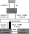
\includegraphics[width=14em]{\chapterdirectory/../cache_coherence/figure/cmp_overview.pdf}
\caption{Vue d'ensemble}%
\label{fr:fig:cache-coherence-cmps-overview}
\end{subfigure} &
\begin{subfigure}[t]{0.47\textwidth}
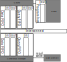
\includegraphics[width=20em]{\chapterdirectory/../cache_coherence/figure/cmp_detailed.pdf}
\caption{Vue comprenant les FIFOs}%
\label{fr:fig:cache-coherence-cmps-fifos}
\end{subfigure}
\end{tabular}
\end{center}
\caption{Composants ayant un rôle dans la cohérence de cache}%
\label{fr:fig:cache-coherence-cmps}
\end{figure}


\begin{definition}[Élément mémoire]
  \label{fr:def:memoryelement}
  La mémoire d'un système est découpée en blocs adressables.
Dans la suite, un élément mémoire correspondra directement à un bloc mémoire.
L'ensemble de tous les éléments mémoire est défini par $\memoryelements{}
\subseteq \mathbb{N}$.
\end{definition}

La cohérence de cache est activée lors des accès à des données partagées et donc lors des exécutions des
instructions d'écriture (\storeinstr{}), lecture (\loadinstr{}) et éviction (\evictinstr{}).

\begin{definition}[Programme s'exécutant sur un c\oe ur]
Les opérateurs élémentaires sont $\operators{} = \{\loadinstr{},
\storeinstr{}, \evictinstr{}, \nopinstr{}\}$ et les instructions considérées
sont
$\instructions{} = \operators{} \times \memoryelements{}$.
Un programme est une séquence d'instructions
et donc $\programs{} =
\sequenceof{\instructions{}}$.
\end{definition}
La notion de séquence sera largement réutilisée dans la suite.
\begin{definition}[Séquence]
\sequenceof{$A$} indique une séquence finie (potentiellement vide)
composée d'éléments de type $A$. Les séquences sont donc définies par:
\[
   \sequenceof{A} =
      \begin{cases}
         \lbrack ~~ \rbrack\\
         A :: \sequenceof{A}
      \end{cases}
\]
L'ajout d'un élément $e$ en tête de la séquence $S$ est noté
\pushfun{$e$}{$S$} et correspond à $e :: S$. L'extraction de la tête de la
séquence $S$ est notée \popfun{$S$}, ce qui retourne $head(S)$ avant d'appliquer
$S \gets tail(S)$. Enfin, \isemptyfun{$S$} indique si $S$ est une séquence
vide et est l'équivalent de vérifier si $S = \lbrack ~~ \rbrack$.
\end{definition}


Les caches sont chargés d'obtenir des copies des éléments mémoire afin de
répondre aux requêtes d'accès mémoire de leur cœur.


\begin{definition}[Ensemble des caches]
\label{fr:def:cache}
L'ensemble des caches du système est défini  par \caches{}.
On note $\cachesandcmgr{} = \caches{} \cup \{\cmgr{}\}$ l'ensemble des caches et le gestionnaire
de cohérence (\cmgr{}).
\end{definition}
Pour gérer les requêtes du c\oe ur,
le cache doit de stocker les
permissions sur chaque élément mémoire
et les opérations en cours.
Pour obtenir de nouvelles permissions, un cache envoie des demandes sur
l'interconnect afin de se coordonner avec les autres caches et le gestionnaire de cohérence.
Chaque demande ne concerne qu'un seul élément mémoire.
On considèrera les demandes de copie en lecture seule
de l'élément mémoire (\getsquery, faisant généralement suite à une instruction
de \loadinstr{}); de copie en écriture et lecture (\getmquery,
faisant généralement suite à une instruction de \storeinstr{}); et le signalement
d'une éviction pour un élément mémoire ayant potentiellement été modifié
(\putmquery, faisant généralement suite à un \evictinstr{}).

\begin{definition}[Demande]
Il existe trois catégories de demande $\queries{} = \{\getsquery,
\getmquery, \putmquery\}$.
Un message envoyé sur l'interconnect pour émettre une demande est défini par
$\querymessages{}: \queries{} \times \memoryelements{} \times \caches$, qui
indique le type de la demande, l'élément mémoire visé et l'émetteur du message.
\end{definition}

Chaque demande fera l'objet d'une réponse.
Une réponse peut simplement contenir une copie de l'élément mémoire (\simpledata);
une réponse peut indiquant qu'aucun autre cache ne possède actuellement de copie de cet élément
mémoire (\exclusivedata); et une réponse peut informer qu'aucune copie ne sera
envoyée (\nodata).


\begin{definition}[Réponse]
Il existe trois catégories de réponse $\replies{} =
\{\simpledata,
\allowbreak{}
\exclusivedata,\allowbreak{} \nodata\}$.
Un message envoyé sur l'interconnect pour émettre une réponse est défini par
$\replymessages{}:
\replies{} \times \memoryelements{} \times \cachesandcmgr{}$, qui indique la
catégorie, l'élément mémoire en question, et le cache visé.
\end{definition}

Il est possible que des caches reçoivent des demandes auxquelles ils doivent répondre alors qu'ils
n'ont pas encore reçu les informations nécessaires.
Ils auront donc en charge de gérer toute cette complexité et répondre à l'ensemble des requêtes et demandes qui leur sont envoyées.
Chaque cache a quatre  FIFO, chacune gérant soit la réception ou l'émission
des demandes et des réponses, comme le montre la
Figure~\ref{fr:fig:cache-coherence-cmps-fifos}.

Le gestionnaire de cohérence est un élément central, non nécessairement implanté par un composant unique dans l'architecture,
permettant la coordination entre les caches.
Tout comme les caches, il utilise des files FIFOs pour
gérer les messages entrant et sortant.
L'interconnect connecte notamment les caches et le gestionnaire de
cohérence. Il broadcast les demandes des caches à tous les composants connectés,
y compris le cache émetteur. Les réponses, quant à elles, ciblent
un seul composant et ne sont donc reçues que par celui-ci.

\subsection{Cohérence de cache}
\label{fr:sec:cache_coherence_msi}
Cette partie, inspirée des principes de \cite{Sorin:2011:PMC:2028905},
introduit la cohérence de cache.
Un système avec cohérence de cache est un système dans lequel des applications
utilisant des caches séparés ne perçoivent pas cette séparation lorsqu'elles
lisent et écrivent sur les éléments mémoire.
\begin{property}
  \label{fr:prop:system_wide_value}
Un protole doit vérifier les propriétés suivantes:
\begin{enumerate}
   \setlength{\itemsep}{0pt}%
   \setlength{\parskip}{0pt}%
  \item Les caches ont la valeur système :
    À tout moment, pour chaque élément mémoire, toutes les copies du même élément
mémoire présentes dans un cache ont la même valeur. Cette valeur correspond à
la dernière qui a été écrite pour cet élément mémoire, quel que soit le cache
qui a fait l'écriture.
  \item
    Un seul écrivain ou seulement des lecteurs :
    À tout moment, pour chaque élément mémoire, il y a soit un seul cache autorisé
à écrire et il est aussi le seul à pouvoir lire, soit aucun cache autorisé à
écrire et un nombre indéterminé de lecteurs.
\item
  Garder le fil :
Si un élément mémoire n'a pas de copie en cache, alors la valeur qui se trouve
dans la mémoire principale du système est la dernière à avoir été écrite.
\end{enumerate}
\end{property}


%\stopallthesefloats
\begin{figure}[hbtp]
   \begin{center}
     \begin{subfigure}[b]{0.5\linewidth}
       \resizebox{\linewidth}{!}{
      \begin{tikzpicture}[->,>=stealth',shorten >=1pt,auto,node distance=5cm,
                    semithick]
   \node[state] (I)              {\texttt{I}};
   \node[state] (S) [right of=I] {\texttt{S}};
   \node[state] (M) [below of=I] {\texttt{M}};

   \path[every node/.style={}]
      (I) edge [bend left] node {\textcolor{blue}{\loadinstr{}}?\textcolor{red}{\textcolor{red}{\getsquery{}}}!\textcolor{OliveGreen}{\simpledata{}}?} (S)
      (I) edge [bend right, sloped, anchor=center] node[yshift=-1em] {\textcolor{blue}{\storeinstr{}}?\textcolor{red}{\textcolor{red}{\getmquery{}}}!\textcolor{OliveGreen}{\simpledata{}}?} (M)

      (S) edge node {\textcolor{blue}{\evictinstr{}}?} (I)
      (S) edge [bend right=90, above] node {\textcolor{red}{\textcolor{red}{\getmquery{}}}?} (I)
      (S) edge [bend left, sloped, anchor=center] node[yshift=1.5em] {\textcolor{blue}{\storeinstr{}}?\textcolor{red}{\textcolor{red}{\getmquery{}}}!\textcolor{OliveGreen}{\simpledata{}}?} (M)
      (S) edge [out=430,in=400,looseness=8] node {\textcolor{blue}{\loadinstr{}}?} (S)

      (M) edge [bend left=90, above, sloped] node {\textcolor{red}{\textcolor{red}{\getmquery{}}}?\textcolor{OliveGreen}{\simpledata{}}!} (I)
      (M) edge [bend right=90, above, sloped, anchor=center] node[yshift=-1em] {\textcolor{red}{\textcolor{red}{\getsquery{}}}?\textcolor{OliveGreen}{\simpledata{}}!\textcolor{OliveGreen}{\simpledata{}}!} (S)
      (M) edge [sloped, anchor=center] node[yshift=-1em]
         {\textcolor{blue}{\evictinstr{}}?\textcolor{red}{\putmquery{}}!\textcolor{OliveGreen}{\simpledata{}}!} (I)
      (M) edge [out=230,in=200,looseness=8] node {\textcolor{blue}{\loadinstr{}}?} (M)
      (M) edge [out=280,in=250,looseness=8] node {\textcolor{blue}{\storeinstr{}}?} (M)
   ;
\end{tikzpicture}
}
      \caption{Cache}
      \label{fr:fig:general_msi_cc}
   \end{subfigure}
   \begin{subfigure}[b]{0.3\linewidth}
      \resizebox{\linewidth}{!}{
      \begin{tikzpicture}[->,>=stealth',shorten >=1pt,auto,node distance=5cm,
                    semithick]
   \node[state] (U)              {\texttt{I}};
   \node[state] (M) [left of=U] {\texttt{M}};

   \path[every node/.style={sloped, anchor=center, yshift=1em}]
      (U) edge [bend left] node {\textcolor{red}{\textcolor{red}{\getmquery{}}}?\textcolor{OliveGreen}{\simpledata{}}!} (M)
      (U) edge [loop below] node [below,yshift=-1em] {\textcolor{red}{\textcolor{red}{\getsquery{}}}?\textcolor{OliveGreen}{\simpledata{}}!} (U)

      (M) edge [bend left] node {\textcolor{red}{\putmquery{}}?\textcolor{OliveGreen}{\simpledata{}}?} (U)
      (M) edge [bend left=90] node {\textcolor{red}{\textcolor{red}{\getsquery{}}}?\textcolor{OliveGreen}{\simpledata{}}?} (U)
   ;
\end{tikzpicture}
}
      \caption{Gestionnaire de cohérence}
      \label{fr:fig:general_msi_cmgr}
   \end{subfigure}
   \begin{subfigure}[b]{0.1\linewidth}
 \resizebox{\linewidth}{!}{
     \begin{tikzpicture}[->,>=stealth',shorten >=1pt,auto,node distance=5cm,
                    semithick]
   \node[state] (U)              {};

   \path[every node/.style={sloped, anchor=center, yshift=1em}]
      (U) edge [loop left] node [below,yshift=0.5em] {\textcolor{blue}{\loadinstr{}}!} (U)
      (U) edge [loop right] node [below,yshift=-1em] {\textcolor{blue}{\storeinstr{}}!} (U)
      (U) edge [loop below] node [below,yshift=-1em] {\textcolor{blue}{\evictinstr{}}!} (U)
   ;
\end{tikzpicture}
}
      \caption{Cœur}
      \label{fr:fig:general_msi_cpu}
   \end{subfigure}
   \end{center}
   \caption{Vue d'ensemble du protocole MSI}
   \label{fr:fig:general_msi}
\end{figure}


Le protocole MSI est le protocole élémentaire de cohérence de cache
et les autres protocoles connus en sont en général des extensions.
Le protocole MSI contient trois états stables, qui lui donnent son nom:
\begin{itemize}
  \setlength{\itemsep}{0pt}%
   \setlength{\parskip}{0pt}%
\item \textbf{Modified:}
\textit{Modified}
indique qu'au moins une écriture a été réalisée sur l'élément mémoire. Tant qu'il possède une copie dans cet état, le
cache peut librement lire et écrire. Cela correspond à être l'unique écrivain
dans la Propriété~\ref{fr:prop:system_wide_value}.

\item \textbf{Shared:}
  \textit{Shared}
  correspond à un accès en lecture.

\item \textbf{Invalid:}
\textit{Invalid} indique que le cache ne possède pas de copie
de l'élément mémoire. Il ne peut donc ni le lire ni le modifier en écriture.
\end{itemize}

La Figure~\ref{fr:fig:general_msi} montre les automates correspondant
au cache, au gestionnaire et au c\oe ur. Cette vision est simplifiée
notamment car les FIFO ont été abstraites et les échanges sont synchrones.
Dans les faits, il faut distinguer les états \textit{stables}
ceux représentés ici des états
\textit{transients}, qui
représentent des étapes intermédiaires dans la résolution des demandes et des réponses.

\begin{example}%
\label{fr:ex:general_msi_single_store}
Considérons un système avec deux caches,
$C_A$ and $C_B$, et un seul élément mémoire $E$ tel que, initialement,
$C_A$ n'a pas de copie de $E$ (état \texttt{I}) et $C_B$ a une copie de $E$
dans l'état \texttt{S}. Le gestionnaire de cohérence considère donc $E$
dans l'état \texttt{I}.
Supposons que $C_A$ reçoive une requête de \storeinstr{} de son c\oe ur. Dans cette situation,
$C_A$ envoie une demande \getmquery{}, laquelle est broadcastée aux autres composants.
Voyant le \getmquery{}, $C_B$ doit alors abandonner sa copie de $E$ afin
de maintenir la Propriété~\ref{fr:prop:system_wide_value}.
De son côté, le gestionnaire de cohérence
réagit au \getmquery{} en envoyant une réponse \simpledata{} à $C_A$ et en
considérant désormais $E$ dans l'état \texttt{M}. Cette réponse
\simpledata{} permet à $C_A$ d'obtenir sa copie de $E$ avec un état \texttt{M}
et donc d'exécuter l'instruction du c\oe ur.
\end{example}





\stopallthesefloats

% \section{Objective}
% % 2 pages.
% Un peut tout prendre

\section{Objectif de la th\`ese}

\stopallthesefloats

% \section{Related Works}
% %3 pages en tout.
% \subsection{Benches}
% \subsection{Handling ...}
% \subsection{Formal approaches}

\section{\'Etat de l'art}

\stopallthesefloats

% \section{Identifying cache coherence}
% % 4 pages.

\section{Identifying the Protocol}
The details of cache coherence mechanisms provided in an architecture's
documentation do not go into sufficient details for certification purposes. The
documentation can even be vague enough to cause the applicant to be misled
about which protocol is implemented on the architecture.  To remedy this, the
first contribution made in this thesis is the cache coherence protocol
identification process described in
Chapter~\ref{cha:identifying_cache_coherence}.

\subsection{Summary}
The proposed cache coherence protocol identification process relies on being
able to observe the binary flags defining the state of cache lines, as well as
having sufficient performance monitors to observe cache coherence related
activity (although solutions such as the one presented in
Section~\ref{sec:elusive_hardware_monitors} may provide an alternative). The
general idea being to use the documentation as a basis for the creation of a
detailed hypothetical cache coherence, then validating it against observations
made on the architecture by performing micro-benchmarks. These benchmarks first
perform a reachability analysis on cache states, then the hypothetical cache
coherence is used to generate benchmarks corresponding to behaviors not exposed
by the initial reachability analysis.

Successful application of the proposed strategy results in an ambiguity-free
description of the architecture's cache coherence protocol (meaning a
description following the notations presented in
Chapter~\ref{cha:cache_coherence}).  This ambiguity-free description of the
architecture's cache coherence protocol is an important information to have in
order to prove that the effects of cache coherence on the system are under
control. Indeed, performing benchmarks to measure access latency or bandwidth
without this information is likely to result in the attribution of
characteristics to the application of instructions on an mistaken system state.
For example considering writing speed to be a certain value for memory elements
seemingly in \texttt{Shared} in all caches of the system realizing that the
protocol actually has a \texttt{Forward} state that will improve access speed.

To illustrate the need for cache coherence identification, the case of the NXP
QorIQ T4240 is presented in Chapter~\ref{cha:identifying_cache_coherence}.
This architecture's documentation files indicate a MESI protocol (in the core
documentation \cite{e6500}) with \textit{cache intervention} (in the
motherboard family's documentation \cite{T4240}). By applying of the cache
coherence protocol identification process, the architecture is shown to
implement a MESIF protocol, which is fair from being obvious from the
aforementioned documentation.

\subsection{Limitations}
There are two main limitations to the cache coherence protocol identification
strategy: the risk of an unreasonably large search space during the naive
reachability analysis and the possibility of undetected
behaviors.

The proposed naive reachability analysis performs up to $3 * \cachecount{}$,
benchmarks per observed system state (i.e.~each instruction on each core, if no
caches have the same state). Unfortunately, the number of observed system states
can be needlessly high if the considered binary flags of cache lines contain
quickly changing information not pertinent to cache coherence. For example, if
flags meant to provide information to the cache replacement policy are
unwittingly considered, the number of observed system states is likely to be
exceedingly high.

The other limitation is that it is always possible for the architecture to have
behaviors that were not observed by the benchmarks. Indeed, provided the system
state is actually defined by components that cannot be observed, the naive
reachability analysis might not encounter them. Likewise, nothing can be done
to ensure the benchmarks guided by the hypothetical protocol would expose them
either.

\subsection{Future Works}
The identification process would greatly benefit from the addition of a step
in which the cache's binary flags are analyzed in order to remove what has no
chance of being related to cache coherence.

The \textit{Naught} library currently only performs a single benchmark per
execution. It should be possible to improve it in order to have all benchmarks
for an observable system state be performed in a single execution.

\textit{Naught} could further be improved to perform the complete
identification process in a single execution, if given the ability to look at
the binary flags of cache lines. This would render the application of this
identification process trivial and greatly improve its chances at being adopted
as a common practice.

\stopallthesefloats

% 
% \section{Modeling cache coherence}
% % 4 pages.

\section{Mod\'eliser la coh\'erence de cache}
\label{fr:sec:model}

Cette section offre un aperçu du modèle UPPAAL\footnote{Disponible sur
\url{https://github.com/nsensfel/phylog-cache-coherence}} pour l'analyse des
effets de la cohérence de cache dans les processeurs multi-cœurs. Sont but est
de créer un modèle formel afin de pouvoir faire des analyses automatiques
(décrites dans la Section~\ref{fr:sec:analyze}) tout en assurant que:
\begin{itemize}
  \setlength{\itemsep}{0pt}%
   \setlength{\parskip}{0pt}%
\item Le modèle est aussi générique que possible dans la façon dont il modélise
la cohérence de cache afin de permettre de facilement passer d'un protocole à
un autre.
\item Les protocoles sont modélisés en détails, prenant en compte tous les états
transitoires et sont définis pour des bus \textit{split-transaction}.
\end{itemize}

L'approche choisie est similaire à celles des papiers présentés dans
la Section~\ref{fr:sec:rel_formal}: utiliser un réseau d'automates de
tailles modérées, chacun représentant un composant, afin que le système
résultant soit facile à comprendre et modulaire.

\subsection{Stratégie de modélisation}
\label{fr:sec:modeling:strategy}
% Pour créer un modèle de l'architecture, la solution choisie a été de la baser
% sur les principes expliqués dans la Section~\ref{fr:sec:cache_coherence}.
Le modèle de l'architecture est limité aux éléments directement liés
à la cohérence de cache. On suppose qu'un applicant ayant besoin de
composants plus précis ou de composants additionnels peut soit les
prendre depuis une autre solution, soit intégrer les composants de
cohérence de cache présents ici dans cette autre solution.

Chaque composant a son propre automate. Les états et transitions de chaque automate représentent en premier lieu les communications (via des synchronisations) entre les différents composants. Le fonctionnement interne de chaque composant, comme les états de cohérence, est décrit via des variables d'états qui sont mises à jour dans des fonctions, qui utilisent une
syntaxe proche du C d'UPPAAL. Cela produite des automates plus
petits et plus lisibles, car les transitions sont moins nombreuses et
leur actions sont faites par l'appel à des fonctions au nom
significatif.

\begin{figure}[hbt!]
\begin{center}
\includegraphics[width=0.5\textwidth]{\chapterdirectory/figure/model_overview.pdf}
\end{center}
\caption{Vue d'ensemble des automates du modèle}
\label{fr:fig:UPPAAL:automata_overview}
\end{figure}

La Figure~\ref{fr:fig:UPPAAL:automata_overview} montre tous les automates
définis dans le modèle. On y retrouve les composants d'une architecture multi-coœurs, plus quelques artefacts de modélisation. En effet,
l'interconnect \textit \textit{split-transaction} a été divisé en deux
composantes: un bus de demande et un bus de réponse. De plus, un automate de
file de messages FIFO pour les réponses a été ajouté et est partagé par le
gestionnaire de cohérence et le contrôleur mémoire. Pour finir, un automate
\textit{Urgent Handler} est présent, qui ne correspond à aucun composant
physique mais permet de faire des synchronisations \texttt{urgent}.

% Pour faciliter les communications, un identifiant unique est assigné a certains
% des composants (les caches, les cœurs, le gestionnaire de cohérence, le
% contrôleur mémoire et le bus de demandes). Cet identifiant est utilisé pour la
% sélection du sous canal approprié dans certaines synchronisations, ainsi que
% pour l'identification de l'envoyeur et du receveur des messages. De plus, cela
% permet de préciser dans la déclaration du système à quel automates un automate
% devrait se connecter, en passant l'identifiant des automates cibles comme
% paramètre (par exemple un cache et ses files de messages).

Les transferts de données entre automates sont faits par synchronisation:
l'émetteur stocke la valeur dans une variable globale, qui est lue par le ou
les receveurs. Cette variable globale est définie de manière à clairement
identifier l'émetteur et, s'il y a lieu, le receveur. L'élément mémoire concerné
par l'échange est aussi indiqué dans cette variable globale, ainsi que le type
de message (par exemple \texttt{GetM}). La validité de cette variable globale
n'est assurée que le temps de la transition, puisque la prochaine transition
peut en changer le contenu. En conséquent, les automates la recevant vont
garder une copie du message dans une variable locale.

% \begin{figure}[hbt!]
% \begin{center}
% \begin{tikzpicture}[
  font=\sffamily,
  every matrix/.style={ampersand replacement=\&,column sep=2cm,row sep=2cm},
  source/.style={draw,thick,rounded corners,fill=yellow!20,inner sep=.3cm},
  process/.style={draw,thick,circle,fill=blue!20},
  sink/.style={source,fill=green!20},
  datastore/.style={draw,very thick,shape=datastore,inner sep=.3cm},
  dots/.style={gray,scale=2},
  to/.style={->,>=stealth',shorten >=1pt,semithick,font=\sffamily\footnotesize},
  every node/.style={align=center}]

  % Position the nodes using a matrix layout
  \matrix{
    \node[source] (core0) {Core 0};
      \& \node[source] (cache0) {Cache 0};
      \\

    \node[source] (queryfifo0) {Query FIFO 0}; \& \&
    \node[source] (datafifo0) {Data FIFO 0};
    \\
      \& \node[sink] (databus) {Data Bus}; \&
      \\
      \node[sink] (querybus) {Query Bus}; \&
      \node[sink] (queryfifomgr) {Query FIFO Mgr};\&
      \node[sink] (datafifomem) {Data FIFO Mem};
      \\\\
      \& \node[sink] (cmgr) {Coherence Manager}; \&
      \node[sink] (mem) {Memory};\\
  };

  % Draw the arrows between the nodes and label them.
  \draw[to] (core0) to[bend left=5] node[midway,above] {$CPU\_REQ[0]$} (cache0);
  \draw[to] (cache0) to[bend left=5] node[midway,below] {$CPU\_ACK[0]$} (core0);

  \draw[to] (queryfifo0) to[bend left=5] node[midway,above,sloped] {\!\!\!\!\!\!\!\!$QUERY\_IN[0]$} (cache0);
  \draw[to] (cache0) to[bend left=5] node[midway,below,sloped] {$QUERY\_OUT[0]$} (queryfifo0);
  \draw[to] (datafifo0) to[bend left=5] node[midway,below,sloped] {$DATA\_IN[0]$} (cache0);
  \draw[to] (cache0) to[bend left=5] node[midway,above,sloped] {$DATA\_OUT[0]$} (datafifo0);
%  \draw[to] (daq) -- node[midway,right] {raw event data\\level 1} (buffer);
  \draw[to] (queryfifo0) to[bend left=5] node[midway,above,sloped] {$QUERY\_TO\_BUS[0]$} (querybus);
  \draw[to] (querybus) to[bend left=5] node[midway,above,sloped] {$QUERY\_BROADCAST$} (queryfifo0);


  \draw[to] (datafifo0) to[bend left=5] node[midway,below,sloped] {$DATA\_TO\_BUS$} (databus);
  \draw[to] (databus) to[bend left=5] node[midway,above,sloped] {$DATA\_TRANS[0]$} (datafifo0);
  \draw[to] (datafifomem) to[bend left=5] node[midway,below,sloped] {$DATA\_TO\_BUS$} (databus);
  \draw[to] (databus) to[bend left=5] node[midway,above,sloped] {$DATA\_TRANS[MEM\_ID]$} (datafifomem);

  \draw[to] (cmgr) to[bend left=5] node[midway,above,sloped] {$MEM\_READ$} (mem);
  \draw[to] (cmgr) to[bend right=5] node[midway,below,sloped] {$MEM\_WRITE$} (mem);
  \draw[to] (datafifomem) to[bend right=5] node[midway,above,sloped] {$DATA\_IN[MEM\_ID]$} (cmgr);
  \draw[to] (cmgr) to[bend right=5] node[midway,below,sloped] {$DATA\_OUT[MEM\_ID]$} (datafifomem);

  \draw[to] (querybus) to[bend left=15] node[midway,above,sloped]
  {$QUERY\_BROADCAST$} (queryfifomgr);

  \draw[to] (queryfifomgr) to[bend right=5] node[midway,below,sloped]
  {$QUERY\_IN[MGR\_IN]$} (cmgr);

  \draw[to] (mem) to[bend right=5] node[midway,above,sloped] {$DATA\_OUT[MEM\_ID]$} (datafifomem);
\end{tikzpicture}

% \end{center}
% \caption{Principaux canaux de communication dans le modèle}
% \label{fr:fig:UPPAAL:Comms}
% \end{figure}
% La Figure~\ref{fr:fig:UPPAAL:Comms} montre comment les synchronisations entre
% automates sont organisées. Quelques canaux absents de la figure sont utilisés
% lors de l'initialisation du modèle ou pour forcer une transition à devenir
% \texttt{urgent}.

Le modèle est fait de manière à suivre les suppositions de la
Section~\ref{fr:sec:second_intro} et peut être instancié en configurant les
paramètres listés dans l'Annexe~\ref{app:model_parameters}.

\subsection{Changer de protocole de cohérence}
\label{fr:sec:protocol_switching}

\begin{figure}[hbt!]
\begin{center}
\input{\chapterdirectory/figure/coproswi.tex}
\end{center}
\caption{L'outil \textit{Co(herence) Pro(tocol) Swi(tcher)}}
\label{fr:fig:second_intro:coproswi}
\end{figure}
Afin de rendre le modèle plus facile à adapter à différentes architectures,
celui-ci est accompagné par un outil appelé CoProSwi qui permet de faire un
changement automatique du protocole de cache utilisé.

Comme indiqué dans la Figure~\ref{fr:fig:second_intro:coproswi}, cet outil prend
en entrée un modèle et la description du protocole de cache sous la forme d'un
fichier texte. Cette description correspond aux notations de la
Section~\ref{fr:sec:cache_coherence} et donc aussi à celles du processus
d'identification de la Section~\ref{fr:sec:identify}.

En conséquent, les protocoles décrits pour CoProSwi indiquent notamment:
\begin{itemize}
    \setlength{\itemsep}{0pt}%
   \setlength{\parskip}{0pt}%
% \item
%    Une liste de types de messages.
%    Par exemple \lstinline!(add_data_type DATA_MSG)!.
% \item
%    Une liste de types de demandes Par exemple
%    \lstinline!(add_data_type GET_SHARED)!.
\item La définition du comportement du contrôleur de cache.
\item La définition du comportement du gestionnaire de cohérence.
\end{itemize}

CoProSwi suppose que tous les protocoles sont définis autours des
instructions \loadinstr{}, \storeinstr{} et \evictinstr{}.

Lors de la définition du contrôleur de cache ou du gestionnaire de cohérence:
\begin{itemize}
    \setlength{\itemsep}{0pt}%
   \setlength{\parskip}{0pt}%
\item
   Chaque état de cohérence est déclaré. Ces déclarations indiquent si l'état
   est transitoire ou stable.%  Par exemple,
   % \lstinline!(add_state stable MSI_INVALID)! déclare l'état \textit{Invalid}
   % comme étant stable.
\item
   L'état par défaut des éléments mémoire est aussi indiqué. On considère que cet
   état correspond à la représentation de l'état \textit{Invalid} du protocole.
\item
   Les actions à faire pour chaque état suite à l'observation d'un message ou
   d'une requête du cœur sont clairement définies.
% \item
%    S'il n'y a pas d'actions à faire, l'action \lstinline!(none)! doit être
%    précisée. En effet, l'outil suppose que l'absence d'une liste d'actions est
%    due à une erreur de la part de l'utilisateur.
% \item
%    Le gestionnaire de cohérence de gère que les demandes et les réponses, pas
%    les instructions ou la réception de ses propres demandes (puisqu'il ne peut
%    pas envoyer de demandes).
\end{itemize}

CoProSwi prend donc en charge toutes les difficultés liées à l'adaptation du
modèle à un protocole de cohérence de cache différent. Il n'est donc pas
nécessaire à l'applicant de comprendre le fonctionnement interne du modèle pour
en faire l'usage. CoProSwi est aussi capable de générer la liste exhaustive
de chemins de changement d'états utilisée dans la Section~\ref{fr:sec:identify}.

\stopallthesefloats

% \section{Analyzing cache coherence}
% % 4 pages.
\section{Analyser la coh\'erence de cache}
\label{fr:sec:analyze}
Cette section présente les analyses permettant d'utiliser le modèle de
la section précédente pour mettre en évidence les interférences liées
à la cohérence de cache. Une partie de ces travaux ont été publiés
dans \cite{ecrts19}.

\begin{figure}[hbt]
  \centering
  \resizebox{.7\linewidth}{!}{

\begin{tikzpicture}[->,>=stealth',shorten >=1pt,auto,  semithick, node distance=0.5cm]
\tikzstyle{section} = [state, rectangle, fill=gray!20]
\tikzstyle{result} = [state, rectangle, rounded corners]
\tikzstyle{auxresult} = [state,rectangle,draw=white]
\tikzstyle{input} = [state,rectangle, draw=blue, thick, fill=blue!20, align=center, rounded corners, minimum height=2em]
\tikzstyle{interresult} = [state, rectangle,dashed, rounded corners]

\node[section] (WCETANA)
   {
      \begin{tabular}{@{}c@{}}
         WCET\\
         Analysis\\
         (Section~\ref{sec:analysis:wcet})
      \end{tabular}
   };


\node[auxresult] (SLOWFACTOR) [above right=of WCETANA,yshift=-20pt]
   {
      \begin{tabular}{@{}c@{}}
         Slowdown\\
         Factors
      \end{tabular}
   };

\node[result] (PROGWCET) [below right=of WCETANA,yshift=20pt]
   {
      \begin{tabular}{@{}c@{}}
         WCET of\\
         Programs
      \end{tabular}
   };


\node[interresult,node distance=2cm] (NOSHAREDWCET) [below =of WCETANA]
   {
      \begin{tabular}{@{}c@{}}
         Without Shared\\
         Variables
      \end{tabular}
   };

\node[result] (IMPACTWCET) [xshift=-1cm,yshift=-0.5cm, below right =of NOSHAREDWCET]
   {
      \begin{tabular}{@{}c@{}}
         Impact of\\
         Interference\\
         on WCET
      \end{tabular}
   };

\node[section,node distance=4cm] (HITMISSANA) [right =of WCETANA]
   {
      \begin{tabular}{@{}c@{}}
         Hit \& Miss\\
         Analysis\\
         (Section~\ref{sec:analysis:hit_and_miss})
      \end{tabular}
   };

\node[input] (PARAMEDMODEL) [above =of HITMISSANA]
   {
      \begin{tabular}{@{}c@{}}
         Instantiated\\
         Model
      \end{tabular}
   };

\node[result] (INSTRACCU) [below left =of HITMISSANA,xshift=1cm]
   {
      \begin{tabular}{@{}c@{}}
         Instruction\\
         Accuracy
      \end{tabular}
   };

\node[auxresult] (MEMEACCU) [below right =of HITMISSANA,xshift=-1cm]
   {
      \begin{tabular}{@{}c@{}}
         Mem. Element\\
         Accuracy
      \end{tabular}
   };


\node[section] (INTERCAT) [right =of HITMISSANA,xshift=2.5cm]
   {
      \begin{tabular}{@{}c@{}}
         Interference\\
         Categorization\\
         (Section~\ref{sec:analysis:exposing_interference})
      \end{tabular}
   };

\node[input] (PROTOCOL) [above =of INTERCAT]
   {
      \begin{tabular}{@{}c@{}}
         Cache Coherence\\
         Protocol
      \end{tabular}
   };

\node[interresult] (ANOTPROTO) [below =of INTERCAT]
   {
      \begin{tabular}{@{}c@{}}
         Annotated\\
         Protocol
      \end{tabular}
   };

\node[section] (INSTRIMPA) [below =of ANOTPROTO,xshift=-0.5cm]
   {
      \begin{tabular}{@{}c@{}}
         Instruction Impact\\
         Analysis\\
         (Section~\ref{sec:analysis:missing_link})
      \end{tabular}
   };

\node[result] (RELINSTRINTER) [below =of INSTRIMPA]
   {
      \begin{tabular}{@{}c@{}}
         Relation Between\\
         Instruction \&\\
         Interference
      \end{tabular}
   };

\path[draw,->] (PARAMEDMODEL) -| (WCETANA);
\path[draw,->] ([yshift=-30pt]WCETANA) -- (PROGWCET);
\path[draw,->] ([yshift=30pt]WCETANA) -- (SLOWFACTOR);

\path[draw,->] (PARAMEDMODEL) -- (HITMISSANA);
\path[draw,->] (HITMISSANA) -- (INSTRACCU);
\path[draw,->] (HITMISSANA) -- (MEMEACCU);

\path[draw,->] (PROTOCOL) -- (INTERCAT);
\path[draw,->] (INTERCAT) -- (ANOTPROTO);
\path[draw,->] (ANOTPROTO) -- (INSTRIMPA);
\path[draw,->] (PARAMEDMODEL) -| ([xshift=10pt]INSTRIMPA.north west);
\path[draw,->] (INSTRIMPA) -- (RELINSTRINTER);

\path[draw,->] ([xshift=-20pt]WCETANA) -- ([xshift=-20pt]NOSHAREDWCET);
\path[draw,->] (PROGWCET) -- (IMPACTWCET);
\path[draw,->] (NOSHAREDWCET) -- (IMPACTWCET);
\end{tikzpicture}
}
\caption{Vue d'ensemble des analyses proposées}
\label{fr:fig:analysis:summary}
\end{figure}

Le modèle présenté dans la section précédente comporte des paramètres (par exemple la durée d'un accès à la mémoire) qui doivent être instanciés via une campagne de benchmarks afin de mener les analyses qui sont décrites ici. Ce processus d'instanciation est en dehors du périmètre de la thèse.
La Figure~\ref{fr:fig:analysis:summary} fournit une vue d'ensemble des analyses
proposées. Les rectangles avec fond gris correspondent aux analyses et ceux sans
arrière plan sont les résultats principaux. Les éléments sans bordure sont des
résultats accessoires. Les bordures en pointillés indiquent les résultats
intermédiaires, qui ne sont pas censés être utiles en eux-mêmes.

% Pour que les analyses présentées dans cette section fournissent des informations
% intéressantes à l'applicant, le modèle doit être instancié afin de correspondre
% à l'architecture cible. Cela signifie que les paramètres listés dans
% l'Annexe~\ref{app:model_parameters} ont été définis suite
% à une campagne de benchmarks mesurant la performance.

\begin{figure}[hbt]
\begin{minipage}[c]{0.55\linewidth}
\includegraphics[width=\linewidth]{\chapterdirectory/figure/analysis/model_overview.pdf}
\caption{Aperçu de l'exemple de modèle instancié}
\label{fr:fig:analysis:model}
\end{minipage}
\begin{minipage}[t]{0.2\linewidth}
\begin{enumerate}
  \setlength{\itemsep}{0pt}%
   \setlength{\parskip}{0pt}%
\item \texttt{store 1}
\item \texttt{store 2}
\item \texttt{load 1}
\item \texttt{store 1}
\item \texttt{load 3}
\item \texttt{store 2}
\item \texttt{load 1}
\item \texttt{store 1}
\item \texttt{load 2}
\item \texttt{store 2}
\item \texttt{end}
\end{enumerate}
\caption{Modèle de programme pour Cœur 1}
\label{fr:fig:analysis:demo_prog1}
\end{minipage}
\begin{minipage}[t]{0.2\linewidth}
\begin{enumerate}
  \setlength{\itemsep}{0pt}%
   \setlength{\parskip}{0pt}%
\item \texttt{store 1}
\item \texttt{store 3}
\item \texttt{load 3}
\item \texttt{store 2}
\item \texttt{load 1}
\item \texttt{store 2}
\item \texttt{load 3}
\item \texttt{store 1}
\item \texttt{load 2}
\item \texttt{store 3}
\item \texttt{end}
\end{enumerate}
\caption{Modèle de programme pour Cœur 2}
\label{fr:fig:analysis:demo_prog2}
\end{minipage}
\end{figure}

Le modèle instancié utilisé pour l'illustration des analyses dans cette section
est représenté dans la Figure~\ref{fr:fig:analysis:model}. Celui-ci utilise un
protocole MESI dont les détails sont fournis dans la version complète de la
thèse (voir Figure~\ref{fig:mesi_cc_table}). Le programme
utilisé par chaque cœur est indiqué par les
Figures~\ref{fr:fig:analysis:demo_prog1} et \ref{fr:fig:analysis:demo_prog2}.
Ces modèles instanciés comportent toujours de l'indéterminisme, qui
représente ce que l'applicant ne connaît pas ou ne peut pas contrôler
sur l'architecture.  Par conséquent, le modèle instancié admet
toujours plusieurs traces d'exécution possibles. Les analyses étant
basées sur l'algorithme de model checking d'UPPAAL, toutes ces traces
sont explorées.


\subsection{Analyse de l'impact sur le temps d'exécution}
\label{fr:sec:analysis:wcet}
Cette première analyse regarde les effets de l'interférence sur le temps
d'exécution total des programmes. Notons cependant qu'il s'agit du temps d'exécution calculé sur le modèle
qui peut s'éloigner du temps d'exécution sur l'architecture réelle, notamment en raison des abstractions faites dans la modélisation ou d'une instanciation du modèle insuffisamment précise. 
Les valeurs obtenues sont tout de même intéressantes à comparer avec
d'autres analyses de temps sur un modèle similaire, par exemple pour
le calcul de facteurs de ralentissement (voir
Définition~\ref{fr:def:slowdownfactor}). Par exemple, on peut obtenir
la proportion du temps d'exécution causée par la cohérence de cache en
comparant le modèle avec une version adaptée du même modèle dans laquelle
aucune variable n'est partagée. Bien que cette version adaptée ne soit
probablement pas réaliste, son temps d'exécution peut être utilisé
comme point de référence.

\begin{definition}[Impact de la cohérence de cache sur le temps d'exécution]
Soit $W_{s}$ le temps d'exécution d'un programme sur le modèle instancié, et
$W_{p}$ son temps d'exécution sur une instance du même modèle dans laquelle
toutes les variables ont été rendues privées. La part de $W_{s}$ correspondant
aux mécanismes de cohérence de cache peut être obtenue avec l'équation suivante:
$T_{cc} = W_{s} - W_{p}$
\end{definition}

Pour obtenir les valeurs de $W_{s}$ et $W_{p}$ en utilisant UPPAAL, on emploie
la vérification de modèle. En effet, ces valeurs correspondent au maximum d'une
horloge mesurant le temps d'exécution du cœur étudié. Il est donc possible de la
récupérer avec une formule semblable à\\
\lstinline!sup{not Core1.Terminated}: Core1.runtime!, qui retourne le maximum
pour l'horloge \lstinline!Core1.runtime! dans l'ensemble des états du système
pour lesquels l'automate \lstinline!Core1! n'est pas dans la localité
\lstinline!Terminated!.

\begin{example}[Exemple de mesures de temps d'exécution]
\begin{figure}[hbt]
\centering
\begin{tabular}{|c|c|c|c|c|}
\cline{2-5}
\multicolumn{1}{c|}{}
      & $W_s$ & $W_p$ & $T_{cc}$ & Isolation \\
\hline
Cœur 1 & 2652 & 1102 & 1550 & 702\\
\hline
Cœur 2 & 2452 & 1452 & 1000 & 904\\
\hline
\end{tabular}
\caption{Exemple d'analyse de temps d'exécution}
\label{fr:fig:analysis:wcet_calc}
\end{figure}
La Figure~\ref{fr:fig:analysis:wcet_calc} indique la valeur maximale du temps
d'exécution pour chaque cœur, avec différentes versions de l'exemple du modèle
instancié.
$W_s$ correspond à celle du modèle instancié original (et donc avec les
variables partagées). $W_p$ correspond à celle d'un modèle dans lequel toutes les
variables ont été rendues privées. Ici, on incrémente les adresses d'éléments
mémoires du programme sur le Cœur 2 par $3$ pour éviter tout partage. $T_{cc}$
correspond à la part du temps d'exécution de $W_s$ prise par les mécanismes de
cohérence cache. Enfin, pour montrer un exemple de facteur de ralentissement, on
étudie aussi le cas où chaque programme est exécuté en isolation.
Les résultats de l'analyse sont donc:
\begin{itemize}
    \setlength{\itemsep}{0pt}%
   \setlength{\parskip}{0pt}%
\item
   Cœur 1 souffre d'un facteur de ralentissement de $2652/702 = 3,77$ quand son
   programme tourne en même temps que celui de Cœur 2, comparé à son exécution
   en isolation.
\item
   Cœur 2 souffre d'un facteur de ralentissement de $2452/904 = 2,71$ quand son
   programme tourne en même temps que celui de Cœur 1, comparé à son exécution
   en isolation.
\item
   Exécuter les deux programmes en isolation l'un après l'autre aurait un temps
   d'exécution maximum de $702 + 904 = 1606$ unités de temps.
\item
   Exécuter les deux programmes en parallèle a un temps d'exécution maximal de
   $\max(2652, 2452) = 2652$.
\item
   Exécuter les deux programmes en parallèle mais sans variables partagées a un
   temps d'exécution maximal de $\max(1102, 1452) = 1452$.
\item
   Approximativement $(1550/2652)*100=58,44 \%$  du temps d'exécution de
   Cœur 1 est causé par l'interférence liée à la cohérence de caches.
\item
   Approximativement $(1000/2452)*100=40,78\%$ du temps d'exécution de
   Cœur 2 est causé par l'interférence liée à la cohérence de caches.
\end{itemize}
\end{example}


\subsection{Catégorisation des accès au cache}
\label{fr:sec:cat_cache_access}
Une interférence peut empêcher une instruction de récupérer une valeur dans le cache (parce que son contenu a été modifié récemment à cause d'une autre instruction). C'est ce qu'on appelle un \emph{cache-miss}.
Les analyses de cette
section s'intéressent à la catégorisation des instructions en fonction des \emph{cache-miss} observés. C'est une technique utilisée dans la littérature (voir
Section~\ref{fr:sec:handling_it}).
L'objectif de cette analyse est donc de classer chaque instruction en
tant que \textit{always-hit} (cache toujours prêt),
\textit{always-miss} (cache jamais prêt) ou \textit{uncategorized} (le
cache peut être prêt ou ne pas l'être selon l'exécution). Pour cela,
on utilise l'opérateur de logique temporelle \agop{} afin de s'assurer
que pour toute trace d'exécution du modèle, l'instruction donnée:
\begin{itemize}
    \setlength{\itemsep}{0pt}%
   \setlength{\parskip}{0pt}%
\item Est résolue par le cache immédiatement, dans quel cas l'instruction est
classée \textit{always-hit}.
\item N'est pas résolue par le cache immédiatement et donc
classée \textit{always-miss}.
\item Sinon, on la classe comme \textit{uncategorized}.
\end{itemize}

\begin{example}[Catégorisation des accès au cache]
\label{fr:ex:analysis:instr_chara}
\begin{figure}[hbt]
\begin{center}
\begin{subfigure}[t]{0.45\textwidth}
\centering
\begin{enumerate}
    \setlength{\itemsep}{0pt}%
   \setlength{\parskip}{0pt}%
\item \texttt{store 1} est classé \texttt{AM}.
\item \texttt{store 2} est classé \texttt{AM}.
\item \texttt{load 1} est classé \texttt{UN}.
\item \texttt{store 1} est classé \texttt{UN}.
\item \texttt{load 3} est classé \texttt{AM}.
\item \texttt{store 2} est classé \texttt{AM}.
\item \texttt{load 1} est classé \texttt{AH}.
\item \texttt{store 1} est classé \texttt{AM}.
\item \texttt{load 2} est classé \texttt{UN}.
\item \texttt{store 2} est classé \texttt{UN}.
\end{enumerate}
\caption{Catégorisation pour le Cœur 1}
\label{fr:fig:analysis:demo_chara_prog1}
\end{subfigure}
\begin{subfigure}[t]{0.45\textwidth}
\centering
\begin{enumerate}
    \setlength{\itemsep}{0pt}%
   \setlength{\parskip}{0pt}%
\item \texttt{store 1} est classé \texttt{AM}.
\item \texttt{store 3} est classé \texttt{AM}.
\item \texttt{load 3} est classé \texttt{AH}.
\item \texttt{store 2} est classé \texttt{AM}.
\item \texttt{load 1} est classé \texttt{AM}.
\item \texttt{store 2} est classé \texttt{UN}.
\item \texttt{load 3} est classé \texttt{AH}.
\item \texttt{store 1} est classé \texttt{AM}.
\item \texttt{load 2} est classé \texttt{UN}.
\item \texttt{store 3} est classé \texttt{AM}.
\end{enumerate}
\caption{Catégorisation pour le Cœur 2}
\label{fr:fig:analysis:demo_chara_prog2}
\end{subfigure}
\end{center}
\caption{Exemple de catégorisation des accès cache}
\label{fr:fig:analysis:demo_chara_progs}
\end{figure}
La Figure~\ref{fr:fig:analysis:demo_chara_progs} montre le résultat de la
catégorisation de chaque instruction de notre exemple.
\texttt{AH} correspond à \textit{always-hit}, \texttt{AM} correspond
à \textit{always-miss} et \texttt{UN} correspond
à \textit{uncategorized}.
\end{example}

Cette catégorisation des instructions permet de déterminer quelles
instructions font varier le temps d'exécution. Cependant, certaines de ces
variations ne sont pas liées à la cohérence de cache. Pour
pouvoir répondre au besoin de la certification, il va donc être
nécessaire d'analyser l'interférence elle-même.

\subsection{Catégorisation de l'interférence}
\label{fr:sec:analysis:exposing_interference}
Pour pouvoir comprendre la cause et les effets des interférences générées par
la cohérence de cache, nous proposons de les classifier en fonction de leurs effets
sur le cache affecté. Cette section présente les trois catégories
d'interférences proposées dans cette thèse.

\begin{definition}[Interférence mineure]
On considère qu'un cache subit une interférence mineure lorsqu'il reçoit une
demande en provenance d'un autre cache sans que cette demande ne nécessite
d'actions de sa part. En effet, le cache a alors pris le temps de traiter une
demande sans que cela n'ait eu d'utilité.
\end{definition}

\begin{example}[Interférence mineure]
Le protocole MSI simplifié de la Section~\ref{fr:sec:cache_coherence_msi}
présente des interférences mineures lorsqu'un cache tenant un élément mémoire
dans l'état \texttt{I} reçoit des demandes, ou qu'il reçoit un \texttt{GetS}
(demande d'accès en lecture) alors qu'il a l'élément en \texttt{S}.
\end{example}

\begin{definition}[Interférence de rétrogradation]
On considère qu'un cache subit une interférence de rétrogradation lorsqu'il
perd les permissions d'écriture sur un élément mémoire suite à la demande d'un
autre cache.
\end{definition}

\begin{example}[Interférence de rétrogradation]
Le protocole MSI simplifié de la Section~\ref{fr:sec:cache_coherence_msi}
présente une interférence de rétrogradation lorsqu'un cache tenant un élément
mémoire dans l'état \texttt{M} reçoit une demande \texttt{GetS} de la part d'un
autre cache. En effet, il passe alors à l'état \texttt{S} et perd ses
permissions d'écriture.
\end{example}

\begin{definition}[Interférence d'expulsion]
On considère qu'un cache subit une interférence d'expulsion lorsqu'il perd
toutes ses permissions sur un élément mémoire suite à la demande d'un autre
cache.
\end{definition}

\begin{example}[Interférence d'expulsion]
Le protocole MSI simplifié de la Section~\ref{fr:sec:cache_coherence_msi}
présente des interférences d'expulsion losrqu''un cache tenant un élément mémoire
dans l'état \texttt{S} ou \texttt{M} reçoit une demande \texttt{GetM} (demande
d'accès en lecture et écriture) de la part d'un autre cache. En effet, il passe
alors à l'état \texttt{I} et perd toutes ses permissions.
\end{example}

\subsection{Révéler les interférences liées à la cohérence de cache}
\label{fr:sec:analysis:missing_link}
Pour révéler toutes les interférences causées par la cohérence de
cache en tenant compte des effets catégorisés, il suffit de
faire en sorte que le modèle détecte les cas où l'interférence a
affecté une instruction. Cela permet alors d'utiliser les outils de
model checking d'UPPAAL pour déterminer quelle instruction cause
une interférence sur quelle autre instruction.
Ainsi, cette section identifie les interférences liées à la cohérence de cache en
définissant deux ensembles finis $S_A$ et $S_E$ composés de triplets
$\langle I_o, E, I_t \rangle$, tels que $I_o$ correspond à l'instruction
causant une interférence de type $E$ sur l'instruction $I_T$. L'ensemble
$S_A$ contient les triplets pour lesquels l'interférence est certaine de se
produire alors que $S_E$ correspond à ceux pour lesquels au moins une exécution
présente l'interférence en question.
Combiné avec les résultats de l'analyse de la
Section~\ref{fr:sec:cat_cache_access}, ceci fournit à l'applicant à la fois les
causes et les effets des interférences liées à la cohérence de cache dans le
système modélisé.

\begin{figure}[hbt]
\centering
\begin{tikzpicture}[->,>=stealth',shorten >=1pt,auto,  semithick]
\tikzstyle{instr} = [state,rectangle,  node distance = 1cm and 10cm]
\tikzstyle{cacheline} = [state,rectangle, node distance = 0.5cm and 3cm]

\node[instr] (C1L0)                    {1. \storeinstr{} 1 (AM)};
\node[instr] (C1L1) [below = of C1L0]  {2. \storeinstr{} 2 (AM)};
\node[instr] (C1L2) [below = of C1L1]  {3. \loadinstr{}  1 (UN)};
\node[instr] (C1L3) [below = of C1L2]  {4. \storeinstr{} 1 (UN)};
\node[instr] (C1L4) [below = of C1L3]  {5. \loadinstr{}  3 (AM)};
\node[instr] (C1L5) [below = of C1L4]  {6. \storeinstr{} 2 (AM)};
\node[instr] (C1L6) [below = of C1L5]  {7. \loadinstr{}  1 (AH)};
\node[instr] (C1L7) [below = of C1L6]  {8. \storeinstr{} 1 (AM)};
\node[instr] (C1L8) [below = of C1L7]  {9. \loadinstr{}  2 (UN)};
\node[instr] (C1L9) [below = of C1L8]  {10. \storeinstr{} 2 (UN)};

\node[instr] (C2L0) [right = of C1L0]  {1. \storeinstr{} 1 (AM)};
\node[instr] (C2L1) [below = of C2L0]  {2. \storeinstr{} 3 (AM)};
\node[instr] (C2L2) [below = of C2L1]  {3. \loadinstr{}  3 (AH)};
\node[instr] (C2L3) [below = of C2L2]  {4. \storeinstr{} 2 (AM)};
\node[instr] (C2L4) [below = of C2L3]  {5. \loadinstr{}  1 (AM)};
\node[instr] (C2L5) [below = of C2L4]  {6. \storeinstr{} 2 (UN)};
\node[instr] (C2L6) [below = of C2L5]  {7. \loadinstr{}  3 (AH)};
\node[instr] (C2L7) [below = of C2L6]  {8. \storeinstr{} 1 (AM)};
\node[instr] (C2L8) [below = of C2L7]  {9. \loadinstr{}  2 (UN)};
\node[instr] (C2L9) [below = of C2L8]  {10. \storeinstr{} 3 (AM)};


\path[dashed,every node/.style={sloped, anchor=east}]
   (C2L0) edge [very near end] node [above]{EX} (C1L2)
   (C2L5) edge [very near end] node [above]{EX} (C1L8)
   (C2L8) edge [very near end] node [above]{DE} (C1L9)

   (C1L0) edge [very near end] node [above]{EX} (C2L4)
   (C1L3) edge [very near end] node [above]{EX} (C2L4)
   (C1L5) edge [very near end] node [above]{EX} (C2L5)
   (C1L7) edge [very near end] node [above]{EX} (C2L7)
   (C1L5) edge [very near end] node [above]{EX} (C2L8)
;

\path[every node/.style={sloped, anchor=east}]
   (C2L3) edge [very near end] node [above]{EX} (C1L5)
   (C2L4) edge [very near end] node [above]{DE} (C1L7)



   (C1L4) edge [very near end] node [above]{DE} (C2L9)
;


\end{tikzpicture}

\caption{Interférence dans l'exemple de modèle instancié}
\label{fr:fig:analysis:interference_between_instructions}
\end{figure}

\begin{example}[Interférences dans notre exemple]
  La Figure~\ref{fr:fig:analysis:interference_between_instructions}
  montre les interférences entre les instructions des programmes de
  l'exemple. Les flèches partent de l'instruction générant
  l'interférence. Celles qui sont en pointillés indiquent une
  interférence ne se produisant pas dans certaines des traces
  d'exécution du modèle.  \lstinline!EX! correspond à une interférence
  d'expulsion et \lstinline!DE!  à une interférence de rétrogradation.
  La colonne de gauche correspond au programme de Cœur 1 et celle de
  droite à celui de Cœur 2.  
\end{example}

\stopallthesefloats

%\section{Conclusion}
% % 1 page.
\section{Conclusion}
This chapter has shown how UPPAAL's model checking capabilities can be exploited
to analyze the interference caused by cache coherence on the model from
Chapter~\ref{cha:modeling_cache_coherence}.

This analysis starts by a computation of the WCET for each program. Useful in
itself, this analysis is extended by that of the WCET for these programs with
the architecture in different configurations in order to extract more
information about how much of the execution time is caused by interference.

In order to more precisely understand what determine the WCET and to provide
the user with information about elements of the program that can directly be
manipulated, the analysis proceeds by an categorization of the accuracy of each
instruction. This indicates which instructions are unaffected by the
interference, which instructions are always time-consuming, and which
instructions take a varying amount of time depending on the execution. By
looking at the accuracy of all accesses made on each memory element, patterns
for these instructions of varying execution time can sometimes be found, which
results in a more predictable system.

The determining factor for the accuracy of instructions is then properly
defined. This corresponds to a categorization of all external queries depending
on their effects on the permissions held by a cache, and whether a loss of
permission led to an instruction taking additional time. Thus, three categories
of interference are defined: minor (no change of permission, but loss of time
due to query processing), demoting (loss of writing permission), and expelling
(loss of all permissions).

Finally, analyses are performed in order to determine how each instruction
interfere with the other instructions. This results in a graph showing, for
each instruction, which instruction can generate interference that will
directly impact it, the category of this interference, and whether this
interference occurs on all possible executions or not.

This provides the user with a clear understanding of the causes and effects of
cache coherence interference on the programs' instructions, opening the way to
finding means of mitigation for this interference.

\stopallthesefloats
\end{otherlanguage}
